\section{Introduction}
\label{ch7:sect:introduction}

Generative aerodynamic inverse design is a data-driven approach that leverages generative models to propose high-performance designs. It has emerged as an alternative to traditional discriminative design, which  performs an optimization to find a single optimal solution~\cite{aa.Li2022b, aa.Lyu2024} and relies on a surrogate model for performance estimation. This requires a high-quality initial guess, such as conceptual design, which can be difficult to obtain. In contrast, generative design operates without such dependency and enables a broader exploration of the design space. It does so by learning the implicit distribution of valid aerodynamic shapes from existing data, enabling probabilistic sampling of feasible configurations. Some examples in deep generative models include variational autoencoders (VAEs)~\cite{ai.Kingma2014}, generative adversarial networks (GANs)~\cite{ai.Goodfellow2020}, and flow-based generative models, which rely on \textit{normalizing flows} to define expressive probability distributions from which data are generated~\cite{aa.Papamakarios2021}. With the advancement of flow models for the latter category, such as diffusion models~\cite{ai.Ho2020, ai.Song2021c} and flow matching~\cite{ai.Lipman2022}, the denoising paradigm has enabled more controllable and high-fidelity generative processes. Furthermore, physics-based guidance can be provided during shape generation. This steers the generative process towards generating geometrically valid and high-performance aerodynamic shapes. These may feature non-intuitive innovations beyond traditional parameter limits while still meeting performance goals.

Physics can be incorporated into generative models in two ways: via conditional training or through inference-time guidance, depending on when the physics guidance is introduced. Figure~\ref{ch7:fig:fmStrategy} shows four representative physical guidance strategies of generative design.  
\begin{figure}[htbp]
    \centering
    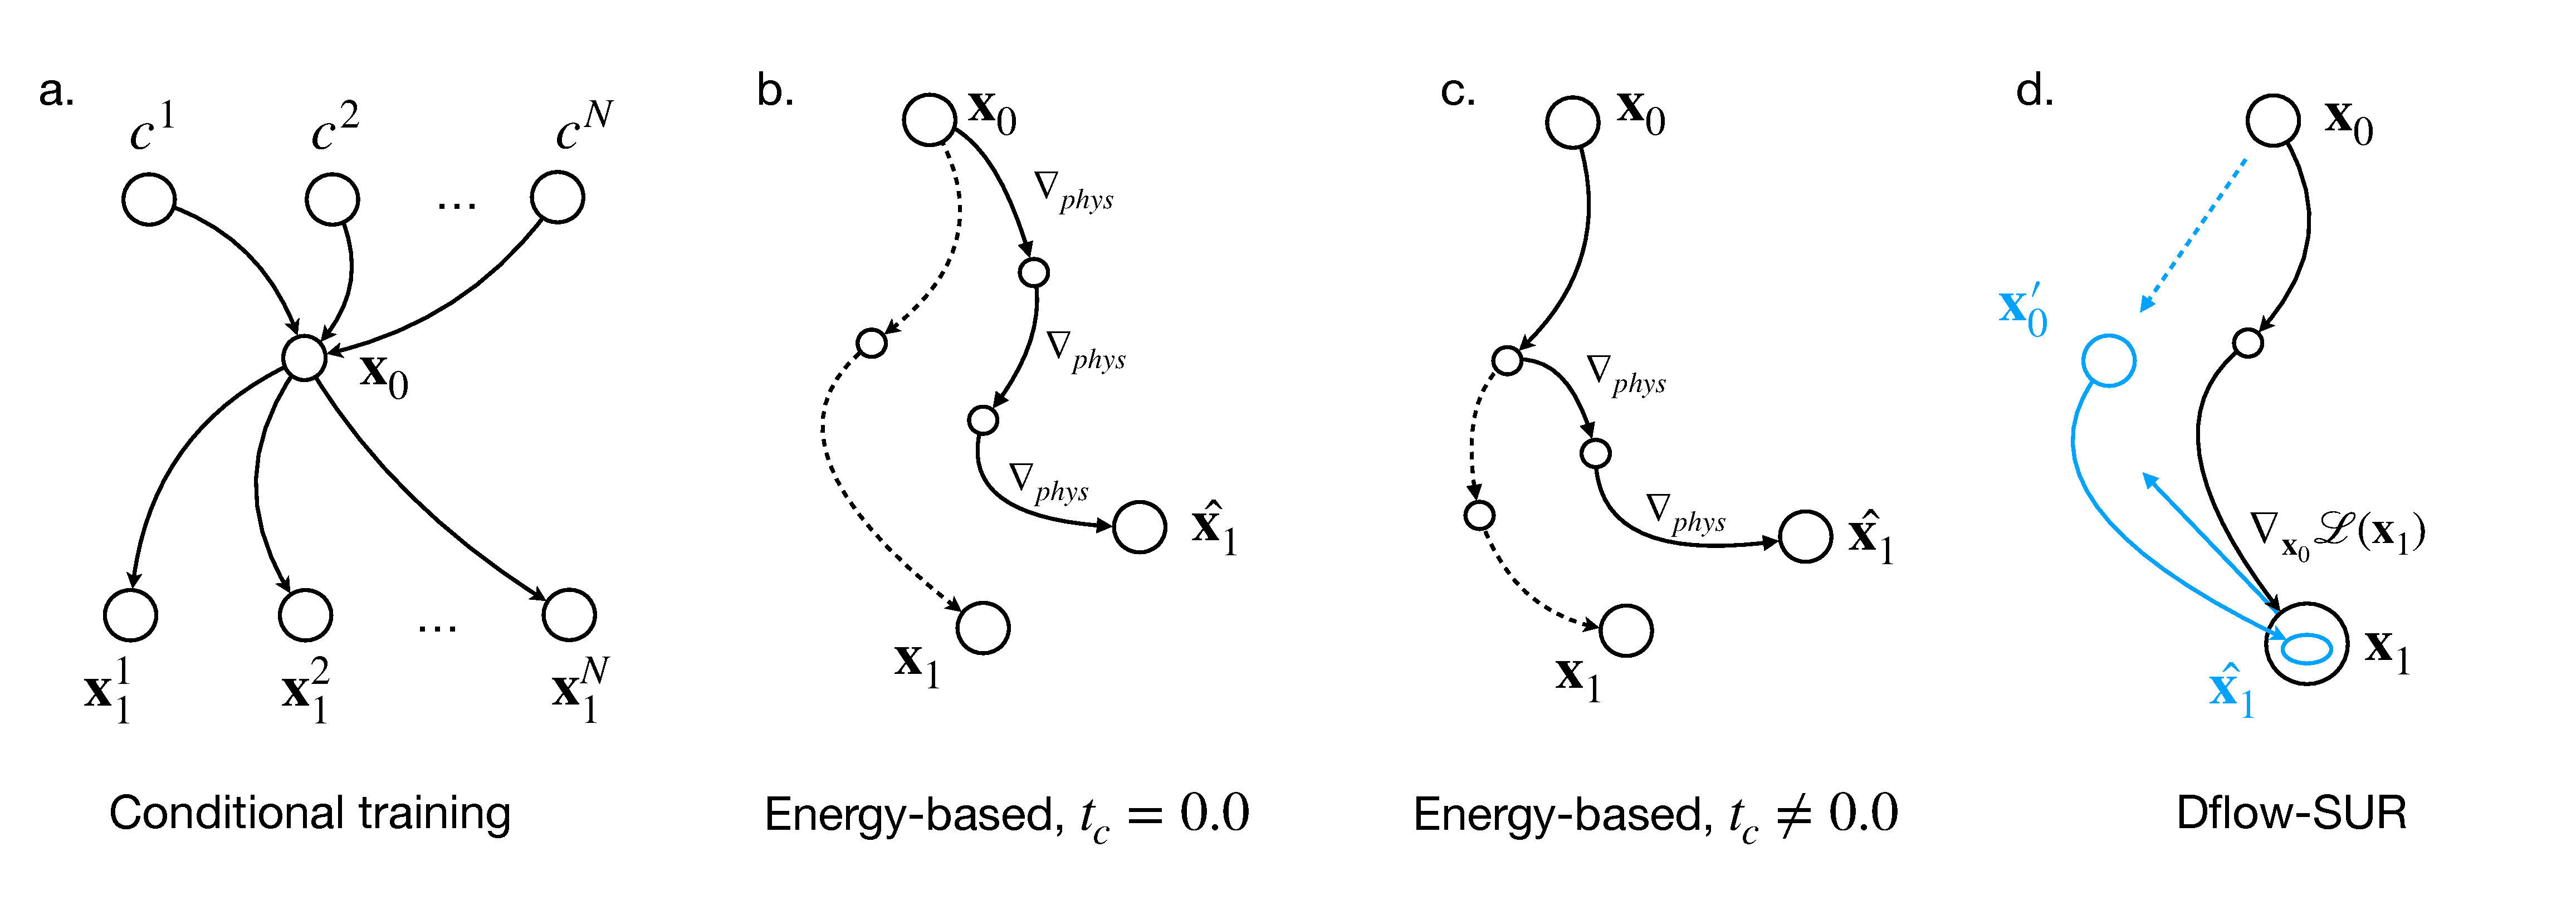
\includegraphics[width=1.0\linewidth]{chapter7/fig/Gen_paper.pdf}
    \caption{Four physical guidance generation strategies: a. conditional guidance during flow matching training; b and c represent energy-based approach with different $t_c$ setting; d is the newly developed \textit{Dflow-SUR}. Strategies shown in b, c, and d involve physical guidance during flow matching inference.}
    \label{ch7:fig:fmStrategy}
\end{figure}
Figure~\ref{ch7:fig:fmStrategy}a depicts the conditional training strategy, where the physical loss $\mathcal{L}_{\mathrm{phys}}$ is combined with the flow matching loss during model training. This strategy has been adopted in previous studies~\cite{aa.Lu2023,aa.Yang2024}. The remaining strategies apply physical guidance during inference: the energy-based approach is shown in Figures~\ref{ch7:fig:fmStrategy}b and \ref{ch7:fig:fmStrategy}c (to be discussed in Section~\ref{ch7:subsubsect:energy}) and the proposed \textit{Dflow-SUR} approach is illustrated in Figure~\ref{ch7:fig:fmStrategy}d (to be detailed in Section~\ref{ch7:subsubsect:diff}).

 % In the inference-time guidance, the flow model is pre-trained unconditionally on the design distribution to obtain a base velocity field, and the physics loss is applied only during generation to steer sampling. 

In conditional training, the physical loss $\mathcal{L}_{\mathrm{phys}}$ is typically combined with the flow-matching loss into a single composite objective, serving as a conditional signal alongside the design $\mathbf{x}$ under which the neural network jointly learns the velocity field parameterization. In the context of aerodynamic inverse design, conditional training has been applied to solve multipoint~\cite{aa.Lin2025} and multifidelity problems~\cite{aa.Yang2024}. Lin~\etal~\cite{aa.Lin2025} implemented a classifier-free conditioning by randomly dropping and concatenating performance targets as inputs during diffusion training so the model learns to generate airfoil shapes both with and without explicit condition guidance, eliminating the need for separate classifier networks. Yang~\etal~\cite{aa.Yang2024} trained a conditional diffusion model by optimizing a score network on noisy shapes given performance targets and a value function network via contrastive learning of predicted target values to guide sampling toward the desired aerodynamic performance. However, this approach is fundamentally constrained by its training paradigm. First, it lacks flexibility, as any modification to design objectives or constraints necessitates retraining the model. Second, accurately modeling both the design space and the underlying physics jointly demands substantially more data, increasing the burden on data collection and model complexity. Third, the conditioning mechanism is limited to low-dimensional settings, where only a few scalar values can be used as auxiliary inputs to the network.

Currently, the prevailing consensus is to introduce physical guidance during the inference phase of flow model. In this framework, a pre-trained, unconditional flow model handles solely geometry sampling, whereas the physical constraint is incorporated at certain inference time. The physics loss is typically cast as an energy model~\cite{ai.LeCun2006}, giving rise to the energy-based approach (Figures~\ref{ch7:fig:fmStrategy}b and~\ref{ch7:fig:fmStrategy}c). In this approach, physical losses are formulated as an energy equation and its gradients are used to guide the flow model during inference. In the engineering design domain, energy-based generative models constitute a new trend, gaining attention for their ability to incorporate physical constraints into the generation process. Wu~\etal~\cite{aa.Wu2024} developed the Compositional Inverse Design with Diffusion Models (CinDM) method, which reframes inverse design as energy minimization via diffusion, compositing multiple diffusion-based energy functions over overlapping subsets of variables. The composite strategy ensures that designs remain in-distribution locally while generalizing to multi-body designs. In the context of topology optimization, TopoDiff~\cite{aa.Maze2023} injects physical information during intermediate inference stages, leveraging low-uncertainty data for physical generation to help control sample quality. To further reduce inference costs, the diffusion optimization models (DOM) developed by Giannone~\etal~\cite{aa.Giannone2023} adopt a trajectory alignment regularizer, which tightly couples diffusion sampling with physics-based optimization steps and kernel relaxations. 

Despite the demonstrated effectiveness mentioned above, the energy-based approach is constrained by two key issues. The core reason is that surrogate models are typically trained on simulation data from clean, idealized geometries, and the limited training data often result in low robustness when faced with more complex or even noisy, perturbed designs. Under such conditions, two main problems emerge: high predictive uncertainty from the surrogate model and strong sensitivity to hyperparameters, such as the injection time $t_c$ and the energy coefficient $\lambda$. All these issues result in a phenomenon we newly find, termed \textit{asynchronous phenomenon}, leading to failed generation. As illustrated in Figure~\ref{ch7:fig:asynchronous}, the finite inference budget from energy-based approach inherently limits physical-loss optimization. An overly short inference time schedule may lead to insufficient physical loss optimization, while an excessively long schedule increases the computational cost of inference. We refer to the inability to synchronize physical-loss optimization with the generative inference process---i.e., when both processes cannot finish at the same time---as an \textit{asynchronous phenomenon}. As a result, one must manually calibrate multiple hyperparameters (such as energy coefficient $\lambda$, inference time steps $T$ and injection time $t_c$, etc.) to ensure that the generated samples follow a reasonable distribution and achieve the desired reduction in physical loss within the allotted inference budget.
\begin{figure}
    \centering
    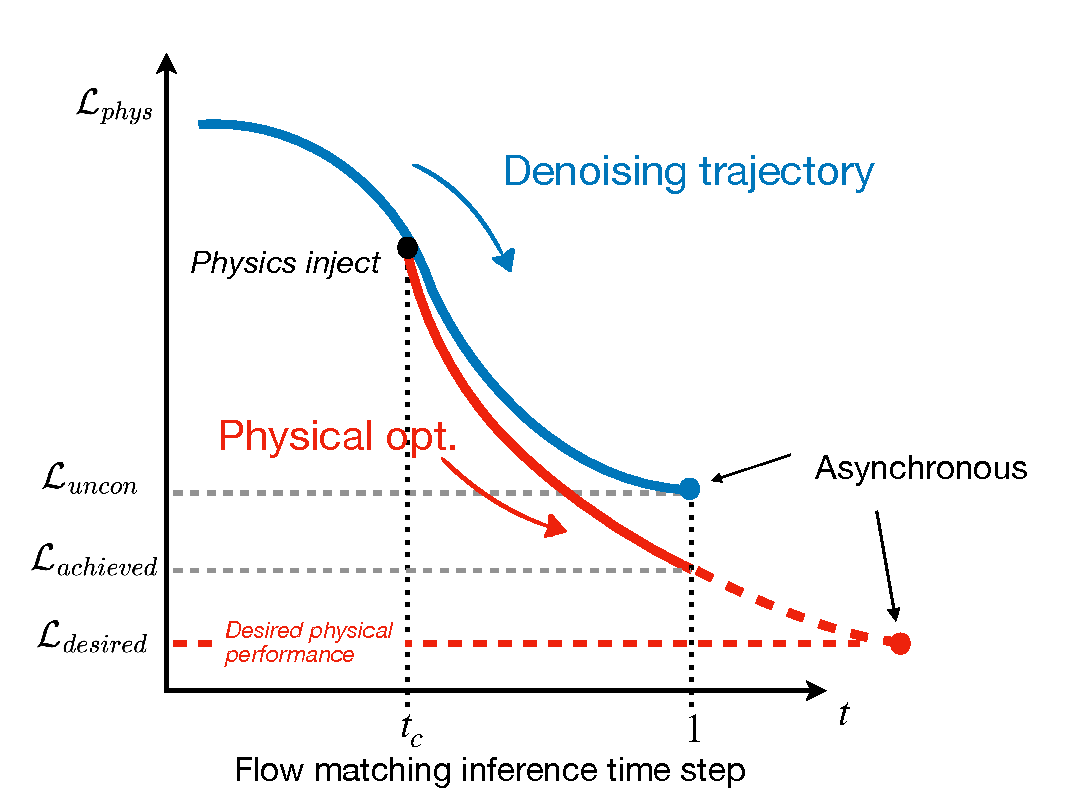
\includegraphics[width=0.75\linewidth]{chapter7/fig/Asynchronous.pdf}
    \caption{Asynchronous dynamics between flow-matching denoising and physical loss optimization. $\mathcal{L}_{\text{uncon}}$ denotes the final physical loss from unconditional generation, $\mathcal{L}_{\text{achieved}}$ represents the final physical loss under energy-based guidance, and $\mathcal{L}_{\text{desired}}$ indicates the target physical constraint imposed on the generative model.}
    \label{ch7:fig:asynchronous}
\end{figure}

To address this issue, we build upon recent advances in differentiable flow matching \textit{D-Flow}~\cite{ai.BenHamu2024} to propose \textit{Dflow-SUR}. It is a decoupled framework that separates inference from physical guidance by updating the generative trajectory using gradients evaluated only on the final generated sample. 
The key contribution of this paper is the demonstration that coupling \textit{D-Flow} with physical surrogate modeling enhances controllability and mitigates uncertainty in surrogate predictions, thereby establishing a significantly more effective generative inverse design framework than previous approaches. 

More specifically, we exhibit through extensive experiments in both conditional training and energy‐based inference, four main strengths of \textit{Dflow-SUR}:
%
\begin{itemize}
    \item \textbf{Superior guidance controllability.} By decoupling the inference dynamics from the physical‐loss gradient, \textit{Dflow-SUR} completely avoids gradient conflicts and thereby improves overall model accuracy.
    \item \textbf{Low surrogate uncertainty evaluation.} In contrast to other methods whose gradients suffer from large surrogate‐model uncertainty at early denoising steps, \textit{Dflow-SUR} confines generation to the data manifold throughout, effectively controlling uncertainty.
    \item \textbf{Hyperparameter robustness.} Whilst existing approaches demand extensive manual tuning of guidance strength to achieve good results, \textit{Dflow-SUR} delivers high-quality designs without any manual adjustment of guidance hyperparameters.
    \item \textbf{Fast and accurate generation.} The decoupled design of \textit{Dflow-SUR} significantly reduces the number of inference time steps while independently optimizing the physical loss, leading to substantial improvements in both computational efficiency and physical accuracy.
\end{itemize}

This paper is organized as follows. In Section~\ref{ch7:sect:relatedWork}, we review the related works. Section~\ref{ch7:sect:methodology} then presents the methodology used in this study, followed by case studies using 2D airfoil and 3D wing presented in Section~\ref{ch7:sect:exp}. Finally,  we conclude the key findings of this work in Section~\ref{ch7:sect:conculsion}.

\section{Related works}
\label{ch7:sect:relatedWork}
The realization of \textit{Dflow-SUR} requires three key components: design representation, physical guidance with a surrogate model, and generative inverse design. We review the related works around these three aspects, which are presented below.

\subsection{Design representation}
Geometry parameterization, as a design representation approach, maps complex geometry into a low-dimensional latent space, enabling efficient learning and optimization while preserving essential features. Control point approaches such as non-uniform rational B-spline (NURBS)~\cite{aa.Systemes2023,aa.Zhao2024} and free-form deformation (FFD)~\cite{aa.Sederberg1986,aa.Hajdik2023} have been shown to be suitable and efficient for design optimization. However, during Design of Experiments (DoE) sampling, control point samples often lie outside the reasonable design space, which disrupts geometric continuity. This shortcoming in turn complicates learning-based optimization by obscuring underlying patterns or constraints. Previous studies have employed data‐subspace techniques—such as singular value decomposition (SVD)~\cite{aa.Masters2017}, proper orthogonal decomposition (POD)~\cite{aa.Wu2019}, and class-shape transformation (CST)~\cite{aa.Kulfan2008}—to render design representations more controllable. For three-dimensional geometries, global‐feature parameterization methods—such as compact modal parameterization~\cite{aa.Li2021c}—have been adopted to capture geometric modes. More advanced approaches such as latent representation method~\cite{aa.Wei2023,aa.Wei2023b} and neural-network-based method~\cite{aa.Wei2024b,aa.Wei2025} have subsequently been introduced to bolster representation robustness and afford greater flexibility by expanding the design’s degrees of freedom. In this study, we employ the CST for airfoil parameterization and the compact modal parameterization scheme for three-dimensional wing geometries, 
which have been shown effective in previous aerodynamic shape optimization studies~\cite{aa.Lyu2024, aa.Yang2025b}. Furthermore, the effectiveness of their derivative computation plugins has also been demonstrated~\cite{aa.Li2021c,aa.Hajdik2023}. 


\subsection{Surrogate-assisted design}
A key enabler in physics-informed generative design is a surrogate model that serves as a fast approximation model to emulate the behavior of expensive physics evaluations~\cite{aa.Liem2015, aa.Li2022b, aa.Paiva2010}. The low-cost gradient information provided by the surrogate model is valuable for rapid conceptual design phases where computational efficiency is critical. The surrogate model construction can be based on Gaussian processes~\cite{aa.Liem2015, aa.Bouhlel2019,aa.Hwang2018}, multi-layer perceptron~\cite{aa.Li2021b}, geodesic convolutional neural networks~\cite{aa.Baque2018}, and transfer learning~\cite{aa.Yang2025} combined with different formations of neural networks, to name a few. By leveraging deep neural networks to enhance the surrogate model, we can push its representation of the physical state toward a higher fidelity level and greater dimensionality on solving complex aerodynamic scenarios, such as wing shape shock mitigation~\cite{aa.Li2021b}, buffet-onset constraint modeling~\cite{aa.Li2022c}, multipoint performance optimization~\cite{aa.Lin2025}, and transonic drag reduction \cite{aa.Zhang2021}. When integrated within a generative modeling, surrogate models can be used during the generation process to impose physics constraints or evaluate candidates on-the-fly without resorting to full simulations. This integration has enabled the exploration of new airfoil designs~\cite{aa.Li2019,aa.Chen2020} and topology structures~\cite{aa.Giannone2023}. In this context, surrogate models offer the advantage of enabling rapid approximation of design variables within the existing data space through high-dimensional interpolation. However, a critical limitation arises in their handling of out-of-distribution (OOD) data, where uncertainty propagates significantly~\cite{aa.Owen2017}.

\subsection{Generative aerodynamic design}
The main purpose of using generative models is to explore new design spaces. Previous approaches such as variational autoencoders (VAEs)~\cite{ai.Kingma2014} and generative adversarial networks (GANs)~\cite{ai.Goodfellow2020} have been used to do shape parameterization (e.g., B\'ezier GAN~\cite{aa.Chen2020}, PaDGAN~\cite{aa.Chen2021b}), geometric filtering~\cite{aa.Li2020}, and accommodate constrained design candidates~\cite{aa.Achour2020,aa.Wang2022,aa.Lei2021}. In recent years, diffusion models~\cite{ai.Ho2020,ai.Song2021c} have emerged as powerful deep generative models with proven performance in computer vision, natural language processing, and modeling of different types of data. This method employs a progressive denoising probabilistic framework that ensures stable training and exact likelihood evaluation, thereby mitigating mode collapse and producing samples with higher fidelity than GANs and VAEs~\cite{ai.Ho2020,ai.Song2021c}. With \textit{DiffAirfoil}, Wei~\etal~\cite{aa.Wei2024} demonstrated diffusion model’s superiority over GANs under data-scarce conditions. In the context of aerodynamic design, our previous study demonstrated the effectiveness of conditional diffusion model as a geometry sampling approach to generate high-fidelity aerodynamic performance wings~\cite{aa.Yang2024}. Several works have also applied conditional diffusion model on multipoint~\cite{aa.Lin2025} and multi-body~\cite{aa.Wu2024} settings in similar design problems. Another generative modeling method is flow matching~\cite{ai.BenHamu2024}, which directly learns a continuous velocity field to map base distribution samples to the target distribution. This method is adopted in this work and will be further discussed in Section~\ref{ch7:subsect:flowBackground}.

